\chapter{Introduction}
  \section{Problématique}
    \lettrine[nindent=0em,lines=3]{L} es systèmes multicoeurs modernes sont
    maintenant basés sur l'architecture NUMA (Non Uniforme Memory Access). Avec
    un système NUMA, les coeurs des processeurs sont regroupés en noeuds. Chaque
    noeud possède un contrôleur mémoire et est interconnecté avec les autres
    noeuds de la machine.
    
    \begin{figure}[H]
      \centering
      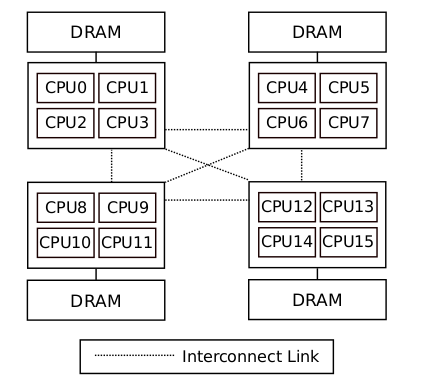
\includegraphics[scale=0.35]{img/numa_arch.png}
      \caption{Un système NUMA avec 4 noeuds et 4 coeurs par noeud}
      \label{f:numa_arch}
    \end{figure}
    
    Du fait des temps d'accès mémoire non uniforme, tout le défi des systèmes
    tournant sur cette architecture est la répartition des données et des
    traitements. En effet, la principale cause de latence n'est pas due au
    \textbf{temps de traitement des données}, mais au \textbf{temps d'accès aux
      données}. Ces accès coûtent entre 10\% et 40\% de temps supplémentaire par
    rapport aux accès locaux.\cite{Lepers2014} Dans une configuration idéale,
    chaque coeur irait chercher ce dont il a besoin dans la mémoire contrôlée
    par le noeud dans lequel il se situe. Ainsi, les demandes d'accès distant
    seraient réduites à néant, et il n'y aurait aucune latence due aux échanges
    entre les noeuds. Nous allons voir que cet idéal est très difficile, voire
    impossible à obtenir. Néanmoins, il est possible de s'en approcher, en
    mettant au point des algorithmes de répartitions de plus en plus
    efficaces. La création de ces algorithmes nécessite une connaissance
    approfondie du noyau: comment gère-t-il la création des threads, où sont-ils
    placés, quelles sont les pages mémoires accédées le plus souvent, par quels
    noeuds sont-elles contrôlées\ldots C'est en collectant un maximum de
    renseignements sur ces différents points (et de nombreux autres) que l'on
    pourra être en mesure d'affiner les solutions de répartition de charge.

    \section{Objectif}
      L'objectif de ce projet a donc été de construire en temps réel une base
      d'informations détaillées contenant les actions des threads les plus
      actifs du système. Cela pour ensuite permettre l'optimisation des accès
      mémoire de manière personnalisée pour chaque thread. La réalisation de cet
      objectif consistait en 3 phases : 

      \bitem
        \item{Etudier et comparer differentes techniques de l'analyse
          d'évènements matériel existantes.}
        \item{Mettre en \oe uvre le mécanisme de mesures matérielles IBS, nous
          avons ainsi pu mesurer les operations les plus importantes effectuées
          par un thread à un moment donné, ces opérations étant les accès
          mémoire distants/locaux, les données envoyées aux autres threads et
          les latences de ces accès mémoire.}
        \item{Elaborer un système de classement en temps réel des threads les
          plus actifs du système, de façon à pouvoir lancer les mesures
          d'évènements sur les threads les plus actifs du noyau et récolter ces
          informations dans des structures de données adaptées.}
      \eitem

  \section{Déroulement}
    Ce projet nous a permis d'avoir accès à la machine Magny Cour (présentée en
    section 2)) située au Laboratoire Informatique de Paris 6, celle-ci
    possédant les caractéristiques adéquates au bon fonctionnement des
    technologies utilisées (présentées en section 3)) pour ce projet.
  
    \paragraph{Phase de démarrage difficile}
      Magny Cour étant utilisée en collaboration avec d'autres chercheurs du
      laboratoire, il n'était pas envisageable de developper et tester notre
      code sur le noyau natif de la machine. La solution a donc été d'utiliser
      des machines virtuelles, le mauvais fonctionnement de la machine virtuelle
      n'interférant pas sur le bon fonctionnement de la machine hôte.\\ Pour ce
      faire nous avons utilisé l'hyperviseur qemu pour lancer des disques
      virtuels contenant nos noyaux modifiés, et dans lesquels nous aurions pu
      lancer des modules faisant tomber en panne la machine virtuelle sans
      conséquences. L'hypothèse de base était donc que les technologies qu'il
      etait question d'utiliser pour effectuer nos mesures seraient simulées par
      qemu. Cette hypothèse s'est révélée fausse, certaines technologies sont
      trop spécifiques au constructeur du processeur. La mise en place de
      l'infrastructure des machines virtuelles (compilation d'un noyau à
      distance, installation d'un noyau compilé, mise en place et utilisation de
      kgdb (debugger de noyau Linux) en mode distant en utilisant des ports
      série) nous a coûté un temps considérable et malheureusement nous n'avons
      pas pu utiliser cette infrastructure pour la plus grande partie du projet,
      les comptages.\\ La deuxième cause du démarrage ralenti de notre projet
      est que globalement les conaissances acquises jusqu'à présent en noyaux,
      processeurs, et mécanismes internes des systèmes d'exploitation n'étaient
      pas suffisantes pour pouvoir utiliser les technologies existantes de
      monitoring en mode noyau.\\ Nous avons donc du lire bon nombre de
      documentations constructeur, d'articles et de sites internet afin de
      comprendre comment mettre en place les mesures. Le but n'était pas
      d'utiliser des librairies qui feraient tout le travail mais d'arriver à
      faire fonctionner nous-même ces mecanismes très bas niveau et d'acquérir
      un maximum de connaissances.

      \paragraph{Comprehension faite, mise en place du comptage}
        Nous avons ensuite pu procéder à l'implémentation des mesures en
        utilisant la technologie IBS (chapitre 3), les tests de fonctionnement
        on donc du se faire sur le noyau natif de la machine Test,
        malheureusement pour comprendre comment marche chaque fonction du noyau
        que nous avons utilisé, il a fallu avancer pas-à-pas et lancer à chaque
        fois le module exécutable, ce qui a très souvent fait planter la
        machine, sans possibilité de redémarrage manuel car nous agissions à
        distance en SSH.

      \paragraph{Classement des threads chauds}
        La troisième partie de la réalisation du projet est une partie où
        pendant la phase de developpement, les test à effectuer ne nécéssitaient
        pas le lancement des mesures, mettre en place un classement des threads
        actifs et les ordonner de manière perfomante pouvait donc se faire dans
        une machine virtuelle, ce que nous avons fait pour limiter l'impact des
        test sur le bon fonctionnement du noyau natif de la machine.

      \paragraph{Merge}
        L'étape finale dans le déroulement du projet a donc été d'associer la
        mise en place du comptage avec le calcul du classement des threads
        actifs, cela a nécéssité d'adapter le code des deux parties et
        d'effectuer quelques mesures.


  \section{Répartition des taches}
    La première partie de compréhension et de mise en place de l'infrastructure
    s'est faite en commun. Ensuite nous nous sommes réparti les taches de la
    manière suivante :

    \bitem
      \item{2 personnes pour la compréhension interne du noyau et des
        processeurs et la mise en place des mesures IBS : Kevin et Pierre-Yves}
      \item{1 personne pour le classement des threads les plus chauds en temps
        réel : Eric}
    \eitem
	
